\documentclass[
  man,
  longtable,
  nolmodern,
  notxfonts,
  notimes,
  colorlinks=true,linkcolor=blue,citecolor=blue,urlcolor=blue]{apa7}

\usepackage{amsmath}
\usepackage{amssymb}




\RequirePackage{longtable}
\RequirePackage{threeparttablex}

\makeatletter
\renewcommand{\paragraph}{\@startsection{paragraph}{4}{\parindent}%
	{0\baselineskip \@plus 0.2ex \@minus 0.2ex}%
	{-.5em}%
	{\normalfont\normalsize\bfseries\typesectitle}}

\renewcommand{\subparagraph}[1]{\@startsection{subparagraph}{5}{0.5em}%
	{0\baselineskip \@plus 0.2ex \@minus 0.2ex}%
	{-\z@\relax}%
	{\normalfont\normalsize\bfseries\itshape\hspace{\parindent}{#1}\textit{\addperi}}{\relax}}
\makeatother




\usepackage{longtable, booktabs, multirow, multicol, colortbl, hhline, caption, array, float, xpatch}
\setcounter{topnumber}{2}
\setcounter{bottomnumber}{2}
\setcounter{totalnumber}{4}
\renewcommand{\topfraction}{0.85}
\renewcommand{\bottomfraction}{0.85}
\renewcommand{\textfraction}{0.15}
\renewcommand{\floatpagefraction}{0.7}

\usepackage{tcolorbox}
\tcbuselibrary{listings,theorems, breakable, skins}
\usepackage{fontawesome5}

\definecolor{quarto-callout-color}{HTML}{909090}
\definecolor{quarto-callout-note-color}{HTML}{0758E5}
\definecolor{quarto-callout-important-color}{HTML}{CC1914}
\definecolor{quarto-callout-warning-color}{HTML}{EB9113}
\definecolor{quarto-callout-tip-color}{HTML}{00A047}
\definecolor{quarto-callout-caution-color}{HTML}{FC5300}
\definecolor{quarto-callout-color-frame}{HTML}{ACACAC}
\definecolor{quarto-callout-note-color-frame}{HTML}{4582EC}
\definecolor{quarto-callout-important-color-frame}{HTML}{D9534F}
\definecolor{quarto-callout-warning-color-frame}{HTML}{F0AD4E}
\definecolor{quarto-callout-tip-color-frame}{HTML}{02B875}
\definecolor{quarto-callout-caution-color-frame}{HTML}{FD7E14}

%\newlength\Oldarrayrulewidth
%\newlength\Oldtabcolsep


\usepackage{hyperref}




\providecommand{\tightlist}{%
  \setlength{\itemsep}{0pt}\setlength{\parskip}{0pt}}
\usepackage{longtable,booktabs,array}
\usepackage{calc} % for calculating minipage widths
% Correct order of tables after \paragraph or \subparagraph
\usepackage{etoolbox}
\makeatletter
\patchcmd\longtable{\par}{\if@noskipsec\mbox{}\fi\par}{}{}
\makeatother
% Allow footnotes in longtable head/foot
\IfFileExists{footnotehyper.sty}{\usepackage{footnotehyper}}{\usepackage{footnote}}
\makesavenoteenv{longtable}

\usepackage{graphicx}
\makeatletter
\newsavebox\pandoc@box
\newcommand*\pandocbounded[1]{% scales image to fit in text height/width
  \sbox\pandoc@box{#1}%
  \Gscale@div\@tempa{\textheight}{\dimexpr\ht\pandoc@box+\dp\pandoc@box\relax}%
  \Gscale@div\@tempb{\linewidth}{\wd\pandoc@box}%
  \ifdim\@tempb\p@<\@tempa\p@\let\@tempa\@tempb\fi% select the smaller of both
  \ifdim\@tempa\p@<\p@\scalebox{\@tempa}{\usebox\pandoc@box}%
  \else\usebox{\pandoc@box}%
  \fi%
}
% Set default figure placement to htbp
\def\fps@figure{htbp}
\makeatother


% definitions for citeproc citations
\NewDocumentCommand\citeproctext{}{}
\NewDocumentCommand\citeproc{mm}{%
  \begingroup\def\citeproctext{#2}\cite{#1}\endgroup}
\makeatletter
 % allow citations to break across lines
 \let\@cite@ofmt\@firstofone
 % avoid brackets around text for \cite:
 \def\@biblabel#1{}
 \def\@cite#1#2{{#1\if@tempswa , #2\fi}}
\makeatother
\newlength{\cslhangindent}
\setlength{\cslhangindent}{1.5em}
\newlength{\csllabelwidth}
\setlength{\csllabelwidth}{3em}
\newenvironment{CSLReferences}[2] % #1 hanging-indent, #2 entry-spacing
 {\begin{list}{}{%
  \setlength{\itemindent}{0pt}
  \setlength{\leftmargin}{0pt}
  \setlength{\parsep}{0pt}
  % turn on hanging indent if param 1 is 1
  \ifodd #1
   \setlength{\leftmargin}{\cslhangindent}
   \setlength{\itemindent}{-1\cslhangindent}
  \fi
  % set entry spacing
  \setlength{\itemsep}{#2\baselineskip}}}
 {\end{list}}
\usepackage{calc}
\newcommand{\CSLBlock}[1]{\hfill\break\parbox[t]{\linewidth}{\strut\ignorespaces#1\strut}}
\newcommand{\CSLLeftMargin}[1]{\parbox[t]{\csllabelwidth}{\strut#1\strut}}
\newcommand{\CSLRightInline}[1]{\parbox[t]{\linewidth - \csllabelwidth}{\strut#1\strut}}
\newcommand{\CSLIndent}[1]{\hspace{\cslhangindent}#1}





\usepackage{newtx}

\defaultfontfeatures{Scale=MatchLowercase}
\defaultfontfeatures[\rmfamily]{Ligatures=TeX,Scale=1}





\title{pairwise interactions on Sicalri's Neural Correlates of Dreaming}


\shorttitle{pySPI Sicalri}


\usepackage{etoolbox}






\author{Arash Sal Moslehian}



\affiliation{
{Neuro-X, EPFL}}




\leftheader{Moslehian}



\abstract{Here I run pyPSI on two electrodes from Siclari's neural
correlates of dreaming paper to see which SPIs perform well for
classifying DE vs.~NE.}

\keywords{information-theory, dreaming, consciousness}

\authornote{ 

\par{       }
\par{Correspondence concerning this article should be addressed to Arash
Sal Moslehian, Email: arash.salmoslehian@epfl.ch}
}

\makeatletter
\let\endoldlt\endlongtable
\def\endlongtable{
\hline
\endoldlt
}
\makeatother
\RequirePackage{longtable}
\DeclareDelayedFloatFlavor{longtable}{table}

\urlstyle{same}



\usepackage{booktabs}
\usepackage{longtable}
\usepackage{array}
\usepackage{multirow}
\usepackage{wrapfig}
\usepackage{float}
\usepackage{colortbl}
\usepackage{pdflscape}
\usepackage{tabu}
\usepackage{threeparttable}
\usepackage{threeparttablex}
\usepackage[normalem]{ulem}
\usepackage{makecell}
\usepackage{xcolor}
\makeatletter
\@ifpackageloaded{caption}{}{\usepackage{caption}}
\AtBeginDocument{%
\ifdefined\contentsname
  \renewcommand*\contentsname{Table of contents}
\else
  \newcommand\contentsname{Table of contents}
\fi
\ifdefined\listfigurename
  \renewcommand*\listfigurename{List of Figures}
\else
  \newcommand\listfigurename{List of Figures}
\fi
\ifdefined\listtablename
  \renewcommand*\listtablename{List of Tables}
\else
  \newcommand\listtablename{List of Tables}
\fi
\ifdefined\figurename
  \renewcommand*\figurename{Figure}
\else
  \newcommand\figurename{Figure}
\fi
\ifdefined\tablename
  \renewcommand*\tablename{Table}
\else
  \newcommand\tablename{Table}
\fi
}
\@ifpackageloaded{float}{}{\usepackage{float}}
\floatstyle{ruled}
\@ifundefined{c@chapter}{\newfloat{codelisting}{h}{lop}}{\newfloat{codelisting}{h}{lop}[chapter]}
\floatname{codelisting}{Listing}
\newcommand*\listoflistings{\listof{codelisting}{List of Listings}}
\makeatother
\makeatletter
\makeatother
\makeatletter
\@ifpackageloaded{caption}{}{\usepackage{caption}}
\@ifpackageloaded{subcaption}{}{\usepackage{subcaption}}
\makeatother

% From https://tex.stackexchange.com/a/645996/211326
%%% apa7 doesn't want to add appendix section titles in the toc
%%% let's make it do it
\makeatletter
\xpatchcmd{\appendix}
  {\par}
  {\addcontentsline{toc}{section}{\@currentlabelname}\par}
  {}{}
\makeatother

%% Disable longtable counter
%% https://tex.stackexchange.com/a/248395/211326

\usepackage{etoolbox}

\makeatletter
\patchcmd{\LT@caption}
  {\bgroup}
  {\bgroup\global\LTpatch@captiontrue}
  {}{}
\patchcmd{\longtable}
  {\par}
  {\par\global\LTpatch@captionfalse}
  {}{}
\apptocmd{\endlongtable}
  {\ifLTpatch@caption\else\addtocounter{table}{-1}\fi}
  {}{}
\newif\ifLTpatch@caption
\makeatother

\begin{document}

\maketitle


\setcounter{secnumdepth}{-\maxdimen} % remove section numbering

\setlength\LTleft{0pt}


\section{Summary}\label{summary}

\begin{itemize}
\item
  I first ran all the SPIs for one subject which took an extremely long
  time to compute. I then removed those SPIs that are computationally
  expensive (see this
  \href{https://github.com/arashsm79/eeg-pairwise-analysis/commit/5046f4e75f1b09937b2b5c9ab8b28e35a6c43362}{commit})
  and the computation time came down to around a minute for each
  recording. The removed SPIs were from Information Theory and Spectral
  connectivity categories. In the end 187 SPIs were left, out of which
  only 124 had memory requirements that my computer could satisfy and
  the rest resulted in out-of-memory errors and NaNs
  Table~\ref{tbl-spistats}.
\item
  Managed to get the SPIs requiring octave and java to compute as well.
\item
  I plotted the channels using the \texttt{HydroCelGSN256v10.sfp} file
  into a 3D space and chose once Oz (15) and one Pz (137) channel (see
  \texttt{siclari.ipynb})
\item
  pySPI is using a quite old version of python (3.9 from 2020) along
  with a bunch of other libraries whose versions are out of date. This
  can get quite annoying if you would want to combine pySPI with other
  packages in the same environment. Nevertheless, I have managed to
  package everything up and make it work in a reproducible manner using
  \href{https://docs.astral.sh/uv/}{uv}.
\item
  Even though some of the SPIs may be undirected, for the sake of
  simplicity, I only took the upper trianglular entry of the 2x2 matrix
  to use as a feature for classification.
\item
  The classification is based on the experiment 1 of the original paper
  Siclari et al.
  (\citeproc{ref-siclariNeuralCorrelatesDreaming2017}{2017}). I wanted
  to see which SPIs can predict Dreaming Experience (DE) vs No
  Experience (NE) better.
\end{itemize}

\begin{table}

{\caption{{SPI stats}{\label{tbl-spistats}}}
\vspace{-20pt}}

\begin{longtable}[]{@{}ll@{}}
\toprule\noalign{}
Category & Count \\
\midrule\noalign{}
\endhead
\bottomrule\noalign{}
\endlastfoot
Successful & 124 \\
NaNs & 55 \\
Constants & 8 \\
\end{longtable}

\end{table}

\section{Results}\label{results}

Similar to the original paper but with less permutation and splits, I do
five random 70/30 splits and check for statistical significance using a
permutation testing method
\href{https://bookdown.org/kmbm92/Applied-Biostats/perm1.html\#permute-to-generate-a-null-distribution}{see}.
This involves fitting 50 null models (by randomly shuffling the labels)
and testing them with cross-validation. Then, I compare the observed
classification performance for each SPI with the combined null
distribution of all SPIs. This gives me p-values, which I adjust for
multiple comparisons by controlling the family-wise error rate at 0.05
using the Bonferroni method Siclari et al.
(\citeproc{ref-siclariNeuralCorrelatesDreaming2017}{2017}).

The class balance seemed okay between the two condition. Nevertheless
the logistic regression model (glm binomial) should help with that as
well.

Based on this method, none of the SPIs were significant as see in
Figure~\ref{fig-stat}. The top performing SPIs are presented in table
Table~\ref{tbl-topacc}.

\begin{figure}[H]

\caption{\label{fig-stat}}

\centering{

\pandocbounded{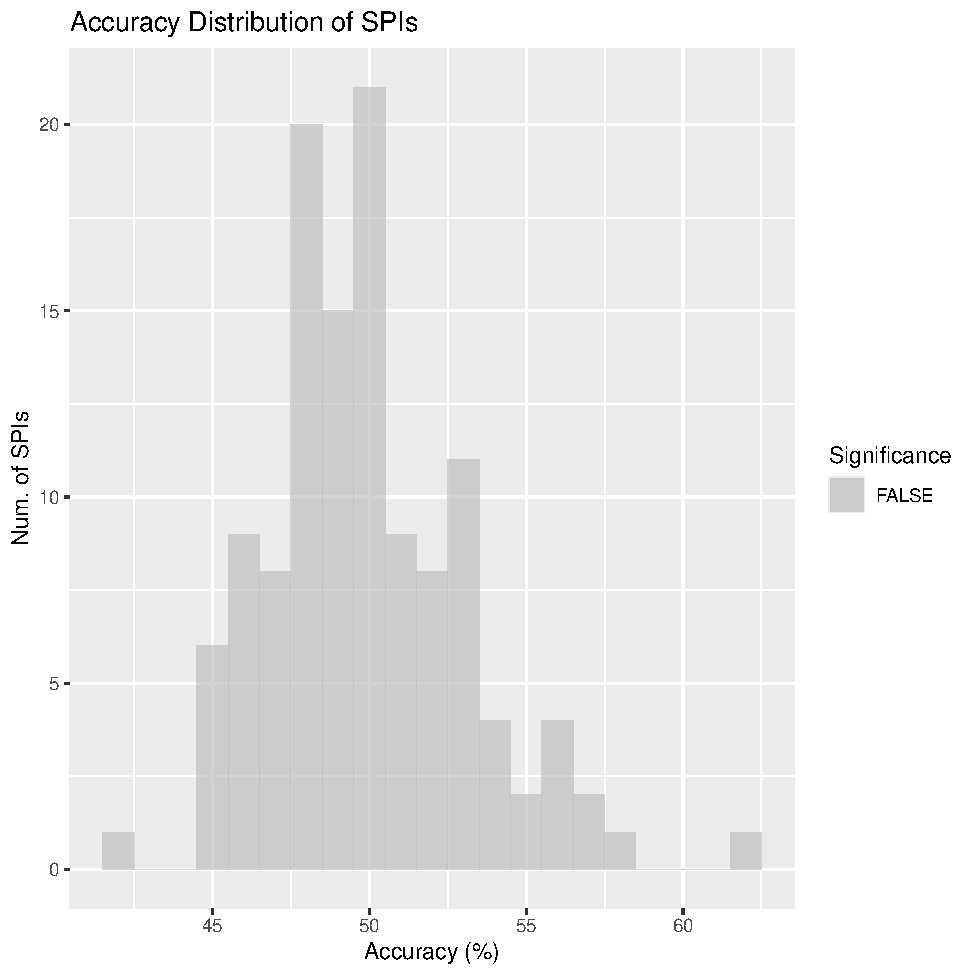
\includegraphics[keepaspectratio]{report_files/figure-pdf/fig-stat-1.pdf}}

}

\end{figure}%

\begin{table}

{\caption{{Top 10 Names}{\label{tbl-topacc}}}
\vspace{-20pt}}

\begin{longtable}[]{@{}llr@{}}
\toprule\noalign{}
& SPI & Accuracy \\
\midrule\noalign{}
\endhead
\bottomrule\noalign{}
\endlastfoot
119 & coint\_johansen\_trace\_stat\_order.1\_ardiff.1 & 0.6227526 \\
1 & cov\_EmpiricalCovariance & 0.5829730 \\
116 & coint\_johansen\_max\_eig\_stat\_order.1\_ardiff.10 & 0.5685107 \\
115 & coint\_johansen\_trace\_stat\_order.0\_ardiff.1 & 0.5676933 \\
118 & coint\_johansen\_max\_eig\_stat\_order.1\_ardiff.1 & 0.5627404 \\
113 & coint\_johansen\_trace\_stat\_order.0\_ardiff.10 & 0.5624172 \\
112 & coint\_johansen\_max\_eig\_stat\_order.0\_ardiff.10 & 0.5570116 \\
76 & psi\_multitaper\_mean\_fs.1\_fmin.0\_fmax.0.25 & 0.5561177 \\
59 & phase\_multitaper\_mean\_fs.1\_fmin.0.25\_fmax.0.5 & 0.5538754 \\
57 & phase\_multitaper\_mean\_fs.1\_fmin.0\_fmax.0.5 & 0.5520878 \\
\end{longtable}

\end{table}

\phantomsection\label{refs}
\begin{CSLReferences}{1}{0}
\bibitem[\citeproctext]{ref-siclariNeuralCorrelatesDreaming2017}
Siclari, F., Baird, B., Perogamvros, L., Bernardi, G., LaRocque, J. J.,
Riedner, B., Boly, M., Postle, B. R., \& Tononi, G. (2017). The neural
correlates of dreaming. \emph{Nature Neuroscience}, \emph{20}(6),
872--878. \url{https://doi.org/10.1038/nn.4545}

\end{CSLReferences}






\end{document}
